\documentclass[conference]{IEEEtran}
\IEEEoverridecommandlockouts
\usepackage{cite}
\usepackage{amsmath,amssymb,amsfonts}
\usepackage{algorithmic}
\usepackage{graphicx}
\usepackage{textcomp}
\usepackage{xcolor}
\usepackage{float}
\usepackage{array}
\def\BibTeX{{\rm B\kern-.05em{\sc i\kern-.025em b}\kern-.08em
    T\kern-.1667em\lower.7ex\hbox{E}\kern-.125emX}}
\begin{document}

\title{Designing a Blockchain-Based Land and Property Registration System in Bangladesh: Technical and Legal Viability}

\author{\IEEEauthorblockN{1\textsuperscript{st} Given Name Surname}
\IEEEauthorblockA{\textit{dept. name of organization (of Aff.)} \\
\textit{name of organization (of Aff.)}\\
City, Country \\
email address or ORCID}
\and
\IEEEauthorblockN{2\textsuperscript{nd} Given Name Surname}
\IEEEauthorblockA{\textit{dept. name of organization (of Aff.)} \\
\textit{name of organization (of Aff.)}\\
City, Country \\
email address or ORCID}
\and
\IEEEauthorblockN{3\textsuperscript{rd} Given Name Surname}
\IEEEauthorblockA{\textit{dept. name of organization (of Aff.)} \\
\textit{name of organization (of Aff.)}\\
City, Country \\
email address or ORCID}
\and
\IEEEauthorblockN{4\textsuperscript{th} Given Name Surname}
\IEEEauthorblockA{\textit{dept. name of organization (of Aff.)} \\
\textit{name of organization (of Aff.)}\\
City, Country \\
email address or ORCID}
\and
\IEEEauthorblockN{5\textsuperscript{th} Given Name Surname}
\IEEEauthorblockA{\textit{dept. name of organization (of Aff.)} \\
\textit{name of organization (of Aff.)}\\
City, Country \\
email address or ORCID}
\and
\IEEEauthorblockN{6\textsuperscript{th} Given Name Surname}
\IEEEauthorblockA{\textit{dept. name of organization (of Aff.)} \\
\textit{name of organization (of Aff.)}\\
City, Country \\
email address or ORCID}
}

\maketitle

\begin{abstract}
    Blockchain technology offers a feasible alternative for transforming land and property registration processes aimed at achieving goals of improved security, transparency, operation efficiency, and reduced corruption. This paper presents the detailed design of a land registration system that is based on blockchain tailored for Bangladesh, where first the technical architecture covering the core components e.g. smart contracts, decentralized ledger systems, and consensus mechanisms are elaborated focusing on ensuring data integrity and availability through comprehensive operational workflows. In addition to the design, this paper also delves into and scrutinizes the legal aspects surrounding blockchain technology that would require intervention by regulators in the Bangladesh legal context. It involves a discussion on property rights, data privacy laws, and the fungibility of digital transactions and records in proving ownership legitimacy. Varieties of successful case studies from countries like Sweden and Georgia which have implemented and pioneered blockchain in land registration are reviewed for their best practices as well as potential challenges to expect. Furthermore, a comparative analysis of the existing land registration process in Bangladesh along with some inefficiencies that could be improved by implementing blockchains are demonstrated in this paper. 
\end{abstract}

\begin{IEEEkeywords}
Null
\end{IEEEkeywords}

\section{Introduction}
Man and property registration policies are basic and important needs to improve a country's economy and ensure the stability of legal systems. The current system that exists in Bangladesh has also several drawbacks, such as inefficiency, and opaqueness that are combined with high risks of fraud and corruption. These problems make secure property rights difficult, if not impossible, to attain – affecting bids for improvements and ownership of land that fuels land disputes and hampers economic advancement and social order. With the country trying to get to the next level in terms of infrastructure and efficient and effective governance, these are historical challenges that require innovation. Blockchain is being viewed as a digital world with no central authority, being highly secure and transparent, and could solve issues of registering land and properties. Thus, when it comes to the application of the given technologies, blockchain in particular, this has the potential of developing a more secure and efficient system that can eliminate as well as minimize the occurrence of fraud as well as enhance the creation of more accurate, secure, and tamper-proof records. The ability to perform such a drastic change in land registries has been acknowledged worldwide and several countries have tested, or adopted, blockchain- based systems for this purpose to gain experience and positive outcomes for further development. Specifically, the research problem that this study is addressing is presented by the existing land and property registration system in Bangladesh – the existing system is ineffective and often invites fraudulent practices and corrupt dealings. These lead to problems such as insecure property rights and frequent issues associated with land issues, which ultimately act as a hurdle in the path of development as well as social justice. To address this, the primary research question is: What kind of change can be implemented to support the land and property registration system in Bangladesh using blockchain technology to increase security, transparency, and efficiency as well as align this solution with the prevailing laws? To realize the aim of this study, several objectives need to be solved. The first objective is to design a centralized blockchain-based land registration system for Bangladesh comprehensively; the technical architecture, main component functionalities, and detailed operational processes are designed in such away that it can accommodate the challenges faced in land registration in Bangladesh. Second, to analyze and explore legal requirements for enforcement and implementation of blockchain technology within Bangladeshi jurisdiction: existing landed laws, property rights law analysis; data privacy regulation, and recognition of digital records must be reviewed to see what extent will be needed changes or additional regulations both at national level as well as regional level. The third objective is to investigate case studies from different countries where blockchain has been used for land registries. By identifying the best practices and potential challenges from an international perspective, the research also assesses how these implications are relevant to Bangladesh. Finally, based on the experiences of other countries and synthesizing evidence, we provide a strategic roadmap for adopting and implementing blockchain for land registrations in Bangladesh. The roadmap will outline some guiding principles that should be followed by policy makers taking into account inputs from technologists and legal experts which can help realize the benefits of modernization of land recording keeping thus securing property rights in Bangladesh. Despite these limitations, this research intends to contribute to filling the existing gap in the literature by providing broader insight into both technical and legal analysis of blockchain technology so that it can develop a strategic plan for adopting and implementing this new technology in Registers of Deeds of Bangladesh. The conclusion and recommendations of this paper will be imperative for the policymakers, and technologist’s jurists, to create awareness, and partnership to reform the land creation and the property rights in Bangladesh. In so doing, this study aims to advance the knowledge base on the implementation of digitization in the context of land registries in developing countries and its quantum leap toward enhanced security, transparency, and efficiency in property rights.

\section{Literature Review}
The authors of this research suggest a blockchain-based method for Bangladesh's safe, open, and permanent land record maintenance. The system, which offers openness, simplicity of access, and quick, affordable solutions, attempts to stop fraud and guarantee that land data stays safe and synced by using Hyperledger Fabric for digital storage. In comparison to current systems, the suggested model offers more security and data privacy, saving time and money on day-to-day operations. The secure registration and maintenance of land ownership records is ensured by the blockchain-based approach, which raises the general efficacy and dependability of land transactions in Bangladesh. The SHA-256 data encryption method is used in this article to present a blockchain system for land deed authentication that guarantees the safe storage, validation, and preservation of pertinent land deed data. To improve efficiency and security, the system incorporates advanced cryptographic techniques including IPFS, public-key cryptography, and Zero Knowledge proof [1]. 
An immutable ownership record that deters fraud is created by the use of blockchain technology, enabling safer property deed transactions. With the use of cutting-edge cryptographic protocols and SHA-256 encryption, the suggested system offers practical answers for confirming land documents, defending property rights, and promoting confidence in real estate transactions [2]. 
This paper presents a novel way to improve the current land registration system by using side-chain technology and Non-Fungible Tokens (NFTs). The suggested solution seeks to improve security, transparency, and confidence in the land registration process by implementing a side-chain similar to IPFS for decentralized data storage and using NFTs on the blockchain to represent properties. NFTs allow land parcels to be uniquely represented on the blockchain, guaranteeing the individuality and ownership of any piece of real estate. Furthermore, decentralized and unchangeable data storage for property is made possible by the incorporation of a side-chain like IPFS, which improves land registration's security and transparency even further. This innovative solution offers a significant upgrade to the existing land registration system, promising improved efficiency, reliability, and trust in property transactions [3].
In the paper, a decentralized application is introduced for registering land deeds through blockchain technology, specifically utilizing the Ethereum network to build and deploy smart contracts. While the paper demonstrates the viability and effectiveness of the suggested methodology for land registry, it raises concerns about the application's ability to ensure the safety of transactions between buyers and sellers or guarantee timely settlements. The utilization of blockchain technology for a secure land registry system is highlighted, emphasizing the incorporation of Ethereum smart contracts for transparent and immutable record-keeping. However, the paper acknowledges the need for further investigation into mechanisms that ensure transaction safety and prompt settlements within the proposed decentralized application [4].
The paper introduces a novel framework utilizing blockchain technology for land registration in Bangladesh, aiming to tackle issues of transparency, centralization, authenticity, and reliability in the process. It compares various blockchain-based land record systems across different countries, emphasizing the proposed framework's relevance and applicability. The study advocates for the adoption of blockchain technology to enhance the land registration process, offering authentic and indisputable ownership rights to individuals in Bangladesh. Overall, the paper develops and proposes a comprehensive framework tailored for implementing land registration via blockchain, contributing to the advancement of land registration practices in the country [5].
The paper investigates the implementation of a secure land registration system using blockchain technology and majority consensus. It highlights that adopting blockchain lowers security issues in land registration processes. Additionally, the study reveals a remarkable 99\% decrease in human record-keeping effort, underscoring the efficiency gains achieved through blockchain utilization for land registration. The blockchain system employs a majority consensus mechanism and utilizes the Proof of Work (PoW) method with SHA256 for improved data security [6].
The paper proposes a blockchain-based distributed ledger framework for vehicle registration and information management, demonstrating its technical viability in Bangladesh. This framework addresses issues inherent in traditional paper-based management systems, ensuring faster and more transparent processes. Notably, the framework employs a hybrid architecture that enhances user experience while maintaining transparency. This creative solution uses blockchain technology to increase efficiency and transparency in Bangladeshi automobile registration and information management systems [7].
The article delineates a blockchain-based land registration system with the goal of enhancing transparency, diminishing fraud, and easing secure property ownership transactions. The suggested approach incorporates a range of technologies such as HTML, CSS, JavaScript, MetaMask, Ganache, and Solidity, in order to enhance the effectiveness, velocity, and transparency of the land registration procedure. Overall, the system modernizes land registration, giving benefits such as increased transparency, reduced fraud, and improved security in property transactions [8].
The article proposes a blockchain-based system for secure land registration in Bangladesh to address limitations of traditional land registration systems. By utilizing blockchain technology, the proposed system offers decentralized storage of data, ensuring secure land ownership records and mitigating disputes. This approach aims to enhance security, reliability, and transparency in land registration processes by securely storing landowner data and minimizing conflicts of land ownership [9].
The article conducts a systematic literature review (SLR) focusing on blockchain technology-related research articles solely focused on Bangladesh. It identifies 13 sectors where Bangladeshi researchers concentrate their efforts and highlights the reasons for Bangladesh's struggle in adopting blockchain technology. The SLR procedure is evidence-based, and article selection is guided by research questions, particularly emphasizing blockchain technology adoption in Bangladesh. However, it underscores the lack of real implementation in Bangladesh for a land registration system, indicating that further exploration is required regarding the legal framework and technical feasibility of such initiatives [10].

\section{Land Registry System for Bangladesh: Methodology}
This section outlines the methodology for developing a blockchain-based land registry system in Bangladesh, incorporating visual diagrams for clarity.

\subsection{System Architecture}
The system will follow a multi-tier architecture, separating concerns for security and scalability.
\begin{itemize}
    \begin{figure}[H]
        \centerline{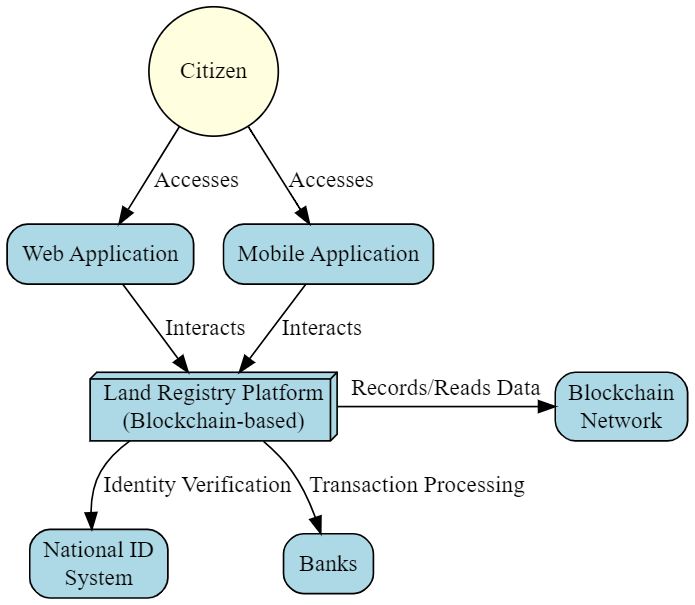
\includegraphics[width=0.8\linewidth]{fig1.png}}
        \caption{System Architecture Diagram.}
        \label{fig1}
    \end{figure}
    \item \textbf{Figure 1} Shows the main components (WebApp, Mobile App, Application Server, Blockchain Network, Database, External Systems) and their interactions.
\end{itemize}

\subsection{Cloud Architecture}
The system will be deployed on a cloud platform (e.g., AWS, Azure, GCP) for flexibility and reliability.
\begin{itemize}
    \begin{figure}[H]
        \centerline{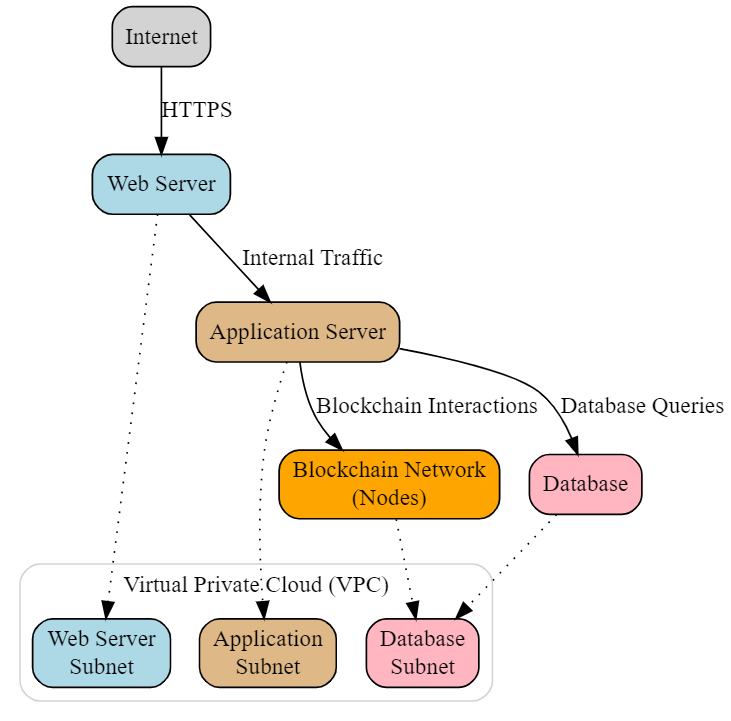
\includegraphics[width=0.8\linewidth]{fig2.png}}
        \caption{Cloud Architecture Diagram.}
        \label{fig2}
    \end{figure}
    \item \textbf{Figure 2} Illustrates the deployment of components within a Virtual Private Cloud (VPC), including subnets for web servers, application servers, and the database.
\end{itemize}

\subsection{Data Modeling}
\begin{itemize}
    \begin{figure}[H]
        \centerline{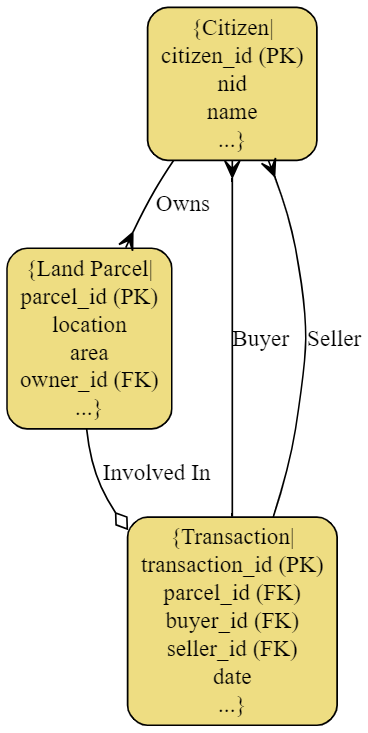
\includegraphics[width=0.4\linewidth]{fig3.png}}
        \caption{Entity Relationship Diagram (ERD).}
        \label{fig3}
    \end{figure}
    \item \textbf{Figure 3} Represents the key entities (Citizen, Land Parcel, Transaction, Document, etc.) and their attributes, relationships, and cardinality.
\end{itemize}

\subsection{Security Design}
Security is paramount. The following measures will be implemented:
\begin{itemize}
    \begin{figure}[H]
        \centerline{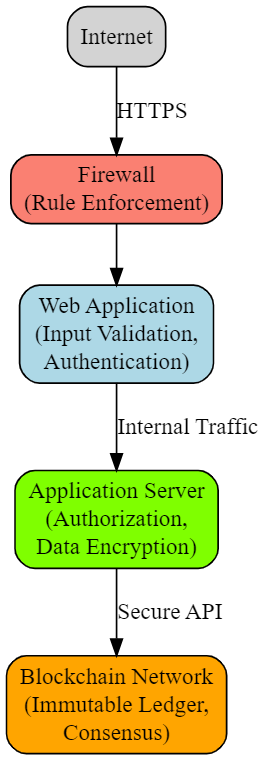
\includegraphics[width=0.3\linewidth]{fig4.png}}
        \caption{Security Diagram (Annotated).}
        \label{fig2}
    \end{figure}
    \item \textbf{Figure 4} Shows security measures integrated into the architecture (firewall, authentication, authorization, data encryption on the App Server, blockchain immutability).
\end{itemize}

\subsection{Process Flows}
\begin{itemize}
    \begin{figure}[H]
        \centerline{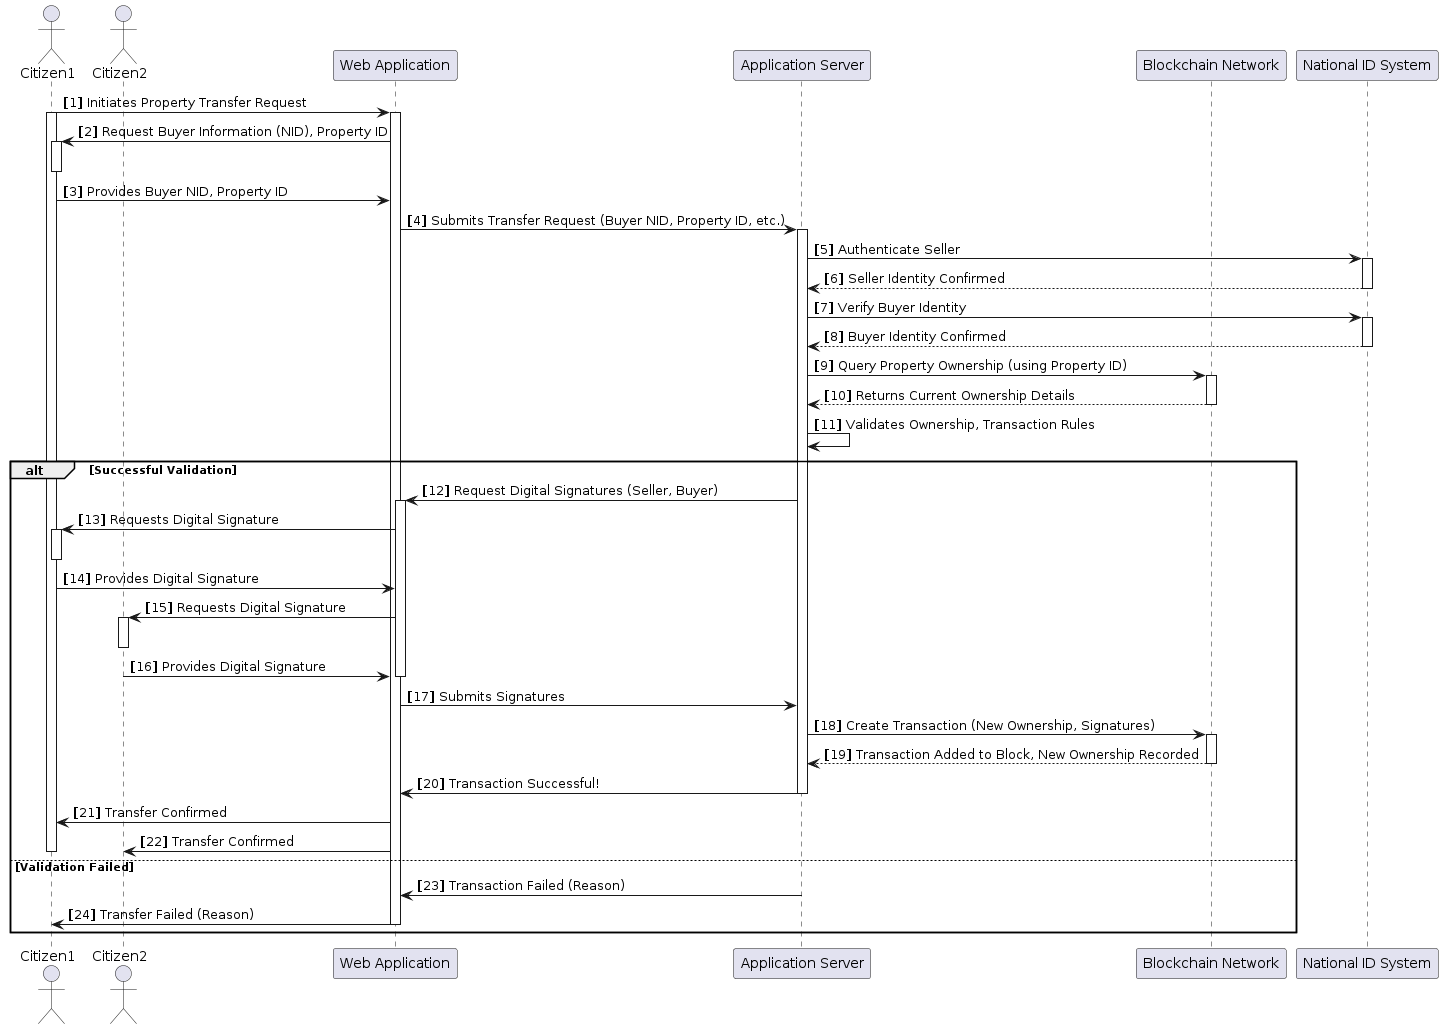
\includegraphics[width=\linewidth]{fig5.png}}
        \caption{Sequence Diagram.}
        \label{fig2}
    \end{figure}
    \item \textbf{Figure 5} Illustrates a detailed sequence diagram for the "Property Transfer" use case. This diagram depicts the message flow and interactions between actors (Seller, Buyer), system components, and the blockchain.
\end{itemize}

\subsection{Deployment \& State Management}
\begin{itemize}
    \begin{figure}[H]
        \centerline{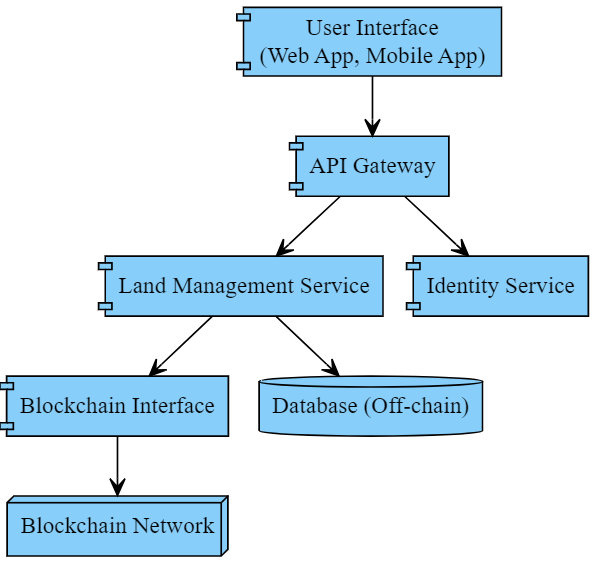
\includegraphics[width=0.8\linewidth]{fig6.png}}
        \caption{Deployment Diagram (Conceptual).}
        \label{fig2}
    \end{figure}
    \item \textbf{Figure 6} Provides a high-level overview of the physical deployment of the system, including the user's devices, network infrastructure, servers, and the blockchain network.
    \begin{figure}[H]
        \centerline{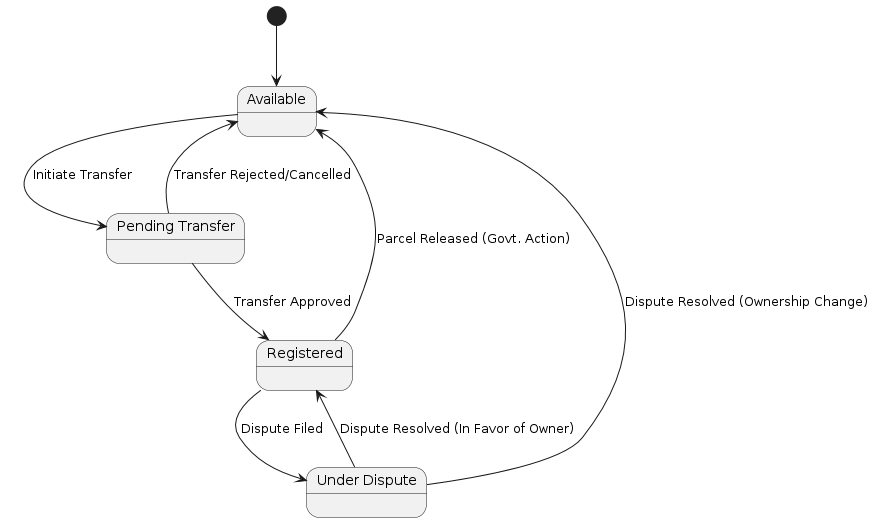
\includegraphics[width=0.8\linewidth]{fig7.png}}
        \caption{Cloud Architecture Diagram.}
        \label{fig2}
    \end{figure}
    \item \textbf{Figure 7} Models the lifecycle of a "Land Parcel" entity, depicting its various states (Available, Pending Transfer, Registered, Under Dispute) and the transitions between them.
\end{itemize}

\subsection{Implementation and Testing}
\begin{itemize}
    \item Use Agile development methodologies with iterative sprints.
    \item Develop and rigorously test each component with unit tests, integration tests, and system tests.
    \item Conduct security audits and penetration testing to identify and address vulnerabilities.
\end{itemize}

\subsection{Pilot and Rollout}
\begin{itemize}
    \item Implement a pilot project in a limited area to gather feedback and refine the system.
    \item Develop training programs for government officials, citizens, and other stakeholders.
    \item Gradually roll out the system nationwide, ensuring widespread adoption.
\end{itemize}

\section*{Comparison of Traditional Land Registration System and Blockchain-Based Proposed System}

The Table \ref{table:comparison} presents a detailed comparison between the traditional land registration system and a proposed blockchain-based system. The comparison is structured to highlight key aspects such as data storage, security, transparency, efficiency, cost, accessibility, fraud prevention, data integrity, regulatory compliance, and scalability.

\begin{table}[H]
    \centering
    \begin{tabular}{|p{1cm}|p{3cm}|p{3cm}|}
        \hline
        \textbf{Aspect} & \textbf{Traditional Land Registration System} & \textbf{Blockchain-Based Proposed System} \\
        \hline
        \textbf{Data Storage} & Centralized, often paper-based or stored in government databases & Decentralized, stored on a blockchain network \\
        \hline
        \textbf{Security} & Vulnerable to tampering, loss, and destruction & Highly secure due to cryptographic techniques and immutability \\
        \hline
        \textbf{Transp- arency} & Limited visibility and prone to corruption & High transparency with public access to transaction history \\
        \hline
        \textbf{Efficiency} & Time-consuming, requires multiple intermediaries & Faster processing with automated smart contracts \\
        \hline
        \textbf{Cost} & High due to manual processes and intermediaries & Lower due to reduced need for intermediaries and automation \\
        \hline
        \textbf{Access- ssibility} & Limited access, often requires physical presence & Global access via the internet, enhancing user convenience \\
        \hline
        \textbf{Fraud Prevention} & High risk of fraud and disputes & Reduced risk of fraud due to immutable records \\
        \hline
        \textbf{Data Integrity} & Susceptible to inconsistencies and errors & Ensured through consensus mechanisms and cryptographic validation \\
        \hline
        \textbf{Regula- tory Compliance} & Requires manual compliance and verification & Automated compliance checks via smart contracts \\
        \hline
        \textbf{Scalab- ility} & Limited by physical and administrative constraints & High scalability due to distributed ledger technology \\
        \hline
    \end{tabular}
    \caption{Comparison of Traditional and Blockchain-Based Land Registration Systems}
    \label{table:comparison}
\end{table}

\section{Legal Viability Analysis}
In a densly populated country like Bangladesh land distribution system is often alleged to foster inequality which goes against fundamental rights and fundamental principles of state policies stated in the Constitution promising to establish economic and social justice.[11]

The blockchain-based documentation procedure as a whole can spare consumers from numerous issues and time-consuming hassles. For example, people won't have to deal with the difficulties of recruiting a document writer to draft their papers. The registration office will automatically receive and generate the records. An agricultural state in India called Andhrapradesh has already effectively implemented this technique, and even the rural populace has benefited from it.

'This state government got rid of -reams of badly maintained paper records, exposed to damage, decay, and tampering—that India's byzantine land-record system can be.The decentralised distributed ledger system—central to cryptocurrencies like bitcoin and ether—has created foolproof digitised land registries of the residential and commercial plots allotted to farmers.'[12]

In general, the traditional land registry system takes an extended period to inspect and requires multiple government authorities to look into this matter. Even in that case, scammers and authorities may manipulate land records.


In this age-old traditional land management and registry system of Bangladesh, most of these laws were made in British Period. These created a system which has created so much lengthy and hectic procedure of Land Registration and management in Bangladesh. Though, It is now 2024 but most if the traditional systems are wholly  unchanged, which has created a corrupted system.

 A study conducted in 2017, was conducted in collaboration with Netherlands based nonprofit The Hague Institute for Innovation of Law (HiiL), the Government of Netherlands, and BRAC. Every year  31 million people face legal dilemmas in Bangladesh.Here land related legal disputes come out on top of the rest. Around 29\% or 8 million people are facing legal problems arise from the land disputes in Bangladesh every year.[13] Thus It's high time to provide people relief from these long time land related disputes by enabling  digitization in land management sector as blockchain system. \\


 1. https://www.printfriendly.com/p/g/iSCm8C\\
 2. https://qz.com/india/1325423/indias-andhra-state-is-using-blockchain-to-build-capital-amaravati\\
 3. https://www.brac.net/latest-news/item/1152-31-million-face-legal-issues-every-year-land-disputes-most-severe / https://www.hiil.org/research/justice-needs-and-satisfaction-in-bangladesh/


\section{Conclusion}

\begin{thebibliography}{00}
\bibitem{b1} Bianca, Gaudenzi. (2023). A Blockchain-Based Secured Land Record System Using Hyperledger Fabric.   doi: 10.1007/978-981-19-8032-9\_13
\bibitem{b2} M.M., Hasan., Md., Mahinur, Alam., Kanita, Jerin, Tanha. (2022). Decentralized Blockchain Based Land Deed Verification and Reservation System in Bangladesh.   doi: 0.1109/ICCIT57492.2022.10054857
\bibitem{b3} Suchithra, M, S. (2023). Implementing a land registration system using non-fungible tokens to represent land in the system and side-chain for data storage.   doi: 10.1109/ICCC57789.2023.10165313
\bibitem{b4} Atul, Lal, Shrivastava., Rajendra, Kumar, Dwivedi. (2023). Blockchain-based Secure Land Registry System using Efficient Smart Contract.   doi: 10.1109/IDCIoT56793.2023.10053476
\bibitem{b5} Sakibul, Islam., Fahmid, Shahriar, Iqbal., Muhaimenul, Islam. (2020). A Novel Framework for Implementation of Land Registration and Ownership Management via Blockchain in Bangladesh.   doi: 10.1109/TENSYMP50017.2020.9230721
\bibitem{b6} Sumit, Kumar, Rana., Sanjeev, Kumar, Rana., Arun, Rana., Sardar, M., N., Islam. (2022). A Blockchain Supported Model for Secure Exchange of Land Ownership: An Innovative Approach.   doi: 10.1109/ICCCIS56430.2022.10037224
\bibitem{b7} Md., Parvez, Hossain., Khaled., Shahjahan, Ahamed, Saju., Shanto, Roy., Milon, Biswas., Muhammad, Aminur, Rahaman. (2020). Vehicle Registration and Information Management using Blockchain based Distributed Ledger from Bangladesh Perspective.   doi: 10.1109/TENSYMP50017.2020.9230781
\bibitem{b8} Galih, Praba, Kusuma., Ch., Rupa., S., R., Juhi, Reshma. (2023). Secure Storage of Land Records and Implementation of Land Registration using Ethereum Blockchain.   doi: 10.1109/ICAIS56108.2023.10073887
\bibitem{b9} Dr.Sangeeta, Gupta., Mohammed, Moazzam, Zahuruddin., Shaik, Waseem, Akram. (2021). Land registration using blockchain technology. Journal of emerging technologies and innovative research.
\bibitem{10} (2022). A Systematic Literature Review of Blockchain Technology Adoption in Bangladesh. Annals of emerging technologies in computing.,  doi: 10.33166/aetic.2022.01.001
\end{thebibliography}

\end{document}
